%!TEX root = ../thesis.tex
%*******************************************************************************
%****************************** Fourth Chapter *********************************
%*******************************************************************************

\chapter{Experimental results}
\label{chap:systml}
\ifpdf
    \graphicspath{{Chapter4/Figs/Raster/}{Chapter4/Figs/PDF/}{Chapter4/Figs/}}
\else
    \graphicspath{{Chapter4/Figs/Vector/}{Chapter4/Figs/}}
\fi


\victor{sur les vrais problèmes ie HIGGS qu'est-ce que ça donne ?}


\section{Failure of domain adaptation} % (fold)
\label{sec:failure_of_domain_adaptation}


\victor{Find out why this is does not work}


\victor{La simulation est trop précise. cf resultat sur l'impossibilité de séparer les domaines créé}


\section{Forest robustness} % (fold)
\label{sec:forest_robustness}

\victor{Grad boost is robust because trees disagrees between themselves}



\section{Explore the theoretical limits}

On va construire un petit jouet 1D qui sur lequel on peut calculer la vraissemblance d'un event $x$.

On va calculer les valeurs théoriques de variance d'autre grandeur et voir ce que ça donne.

L'idée est de pouvoir comparer avec un classifieur, inferno ou la régression directe pour mesurer leur marge de progression possible.

\emph{Hypothèse 1} : on ne peut pas réduire l'erreur systématique complètement

Nos observations $x$ dépendent du paramètre d'intérêt $y$ et des param de nuisance $\alpha$ de façon non triviale.
Il parait raisonnable de penser qu'il n'est pas possible de complètement réduire la dépendance entre $y|x$ et $\alpha$.

\emph{Hypothèse 2} : même avec un classifieur simple (sans adaptation de domaine ou autre) on atteint l'erreur systématique minimum (ou presque)

\emph{Hypothèse 3} : Si H1 et H2 sont vrai alors le mieux à faire pour réduire l'erreur systématique est d'avoir une meilleure connaissance sur les paramètres de nuisance ie améliorer la calibration.

\subsection{Theory} % (fold)
\label{sub:theory}


Définition de la variance :

$\VV(Y) = \EE[(Y - \EE[Y])^2] = \EE(Y^2) - [\EE(Y)]^2$

Théorème de la variance totale \needcite :

\begin{eqnarray}
    \VV[Y] =& \EE_X \left (\VV[Y|X] \right ) &+ \VV_X \left (\EE[Y|X]\right ) \\
    \VV[Y] =& \EE_X \left (\VV[Y|X] \right ) &+ \EE_X \left ( (\EE [Y|X]  - \EE[Y])^2\right )
\end{eqnarray}


En remplaçant la v.a. $Y$ par $y|x$ et $X$ par $\alpha$ on obtient :

$$
\VV[y|x] = \EE_{\alpha \sim p(\alpha|x)} \left (\VV[y|x, \alpha] \right ) + \EE_{\alpha \sim p(\alpha|x)} \left ( (\EE [y|x, \alpha]  - \EE[y|x])^2\right )
$$


On dirait presque que : 
$$\EE_{\alpha \sim p(\alpha|x)} \left ((\EE [y|x, \alpha]  - \EE[y|x])^2\right )$$
représente l'erreur systématique. 
Car c'est l'écart de notre estimation de $y$ sachant $x$ et $\alpha$ par rapport à la moyenne.
Surtout, si $\alpha|x$ est parfaitement connu (ie c'est un dirac) alors ce terme s'annule !

Mais je ne suis pas sûr que l'on puisse dire que
$$\EE_{\alpha \sim p(\alpha|x)} \left (\VV[y|x, \alpha] \right )$$
représente l'erreur statistique.

Mais si ça marche on aurrait une définition claire et précise de ce qu'est l'erreur statistique et l'erreur systématique.


\subsection{Motivation} % (fold)
\label{sub:motivation}

Le régresseur est par construction très sensible à la valeur de $\alpha$ donné ce qui rend le 2 ème terme prépondérant dans le calcul de l'incertitude.

$$\EE_{\alpha \sim p(\alpha|x)} \left ((\EE [y|x, \alpha]  - \EE[y|x])^2\right )$$

Je veux mesurer la valeur minimale possible de ce terme pour savoir s'il reste de la marge de progression.

\subsection{Method} % (fold)
\label{sub:method}



On suppose que l'on peut calculer la vraissemblance $p(x|y_i, \alpha_j)$.

On construit une grille, suffisement fine, parcourant les valeurs possibles $y_i, \alpha_j$.

Th. de Bayes : 
$$
    p(y_i, \alpha_j | x) = \frac{p(x|y_i, \alpha_j) p(y_i, \alpha_j)}{p(x)}
$$

On a donc à partir des 2 tenseurs : 
\begin{itemize}
	\item likelihood : $L_{ij} = p(x|y_i, \alpha_j)$
	\item prior : $K_{ij} = p(y_i, \alpha_j)$ 
\end{itemize}

le tenseur $ R_{ij} = p(x|y_i, \alpha_j) p(y_i, \alpha_j) $ 
qui après renormalisation donne le tenseur posterior $ T_{ij} = p(y_i, \alpha_j | x)$.

À partir de $T_{ij}$ on va calculer les proba marginales :
\begin{itemize}
	\item $p(y_i | x) = \sum_j T_{ij} = Y_i$
	\item $p(\alpha_j | x) = \sum_i T_{ij} = A_j$
\end{itemize}

et ce que doit apprendre notre réseau de neuronne : $p(y_i | x, \alpha_j) = \frac{p(y_i, \alpha_j | x)}{p(\alpha_j | x)} = \frac{T_{ij}}{A_j} = N_{ij}$

On obtient alors les grandeurs qui nous intéressent
\begin{itemize}
	\item $ \VV(y|x) = \VV(y_i, Y_i) $
	\item $ \EE_{\alpha \sim p(\alpha|x)}[ \VV(y|x, \alpha) ] = \sum_j \VV(y|x, \alpha_j) p(\alpha_j | x) = \sum_j \VV_i(y_i, N_{ij}) A_j$
	\item $\EE_{\alpha \sim p(\alpha|x)} \left ((\EE [y|x, \alpha]  - \EE[y|x])^2\right ) = \VV(y|x) - \EE_{\alpha \sim p(\alpha|x)}[ \VV(y|x, \alpha) ] = \VV(y_i, Y_i) - \sum_j \VV_i(y_i, T_{ij}) A_j$
\end{itemize}


\subsection{Remarks} % (fold)
\label{sub:remarks}

\subsubsection{Remarque 1}

Pour les calculs il faut se souvenir que les tenseurs contiennent des proba !

Donc $<y|x>= \EE[y|x] = \sum_i y_i Y_i$ car $Y_i$ ne contient la densité de proba mais pas les valeurs de $y$ !

De même $\VV(y|x) = \sum_i y_i^2 Y_i - <y|x>^2 = \VV(y_i, Y_i)$

\subsubsection{Remarque 2}

Pour la stabilité numérique il convient de travailler en logproba.

En effet $x$ représente un jeu de donnée donc $p(x | y_i, \alpha_j) = \prod_k^N p(x_k | y_i, \alpha_j)$ pour N assez grand.
Ceci va produire des nombre très petit très vite !

On calculera plutôt : $\log p(x | y_i, \alpha_j) = \sum_k^N log p(x_k | y_i, \alpha_j) = \ell(x | y_i, \alpha_j)$

La renormalisation se fera facilement avec un softmax : 
$$ 
    T_{ij} = p(y_i, \alpha_j | x) = \frac{e^{\ell(y_i, \alpha_j| x)} }{\sum_{n,m} e^{\ell(y_n, \alpha_m| x)} }
$$


\subsection{1D toy} % (fold)
\label{sub:1d_toy}

Le toy qui va nous interesser ici est un mélange de 2 distributions, une gamma et une gaussienne, avec une observable 1D $x$.
\autoref{fig:minitoy_distrib} présente la distribution des données pour un tirage de 10000 instances.

Le paramètre d'intérêt est le coef de mélange des 2 distributions $y$.
Le paramètre de nuisance $\alpha$ est un rescaling de l'observable $x$.

Sans $\alpha$ :
$$
    p(x | y) = y \mathcal N(x|a, b) + (1-y) Gamma(x|s, \theta)
$$

Avec $\alpha$ :
$$
    p(x | y, \alpha) = y \mathcal N(x|\alpha a, \alpha b) + (1-y) Gamma(x|\alpha s, \theta)
$$

\begin{figure}[htb]
    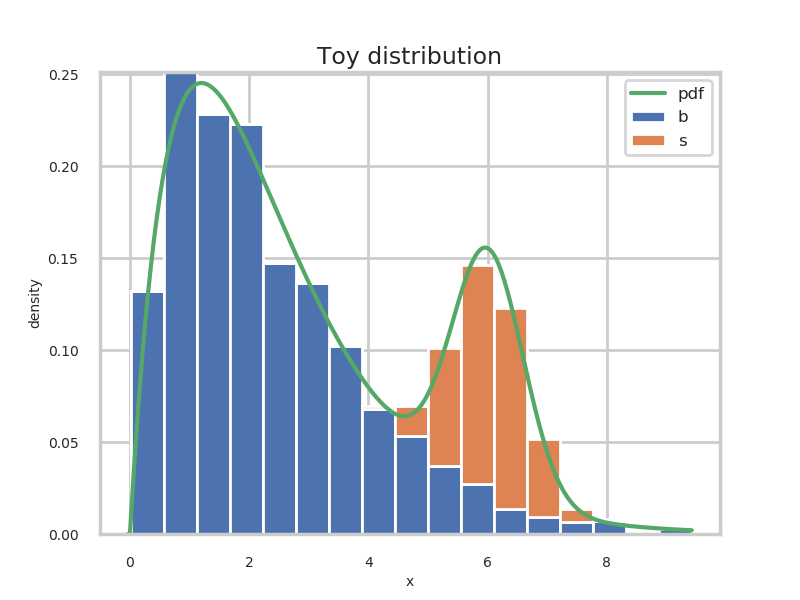
\includegraphics[width=\linewidth]{Chapter4/Figs/Raster/minitoy/distrib.png}
    \caption{Data distribution of the 1D toy}
    \label{fig:minitoy_distrib}
\end{figure}



\begin{figure}[htb]
  \centering
  \begin{subfigure}[t]{0.49\linewidth}
    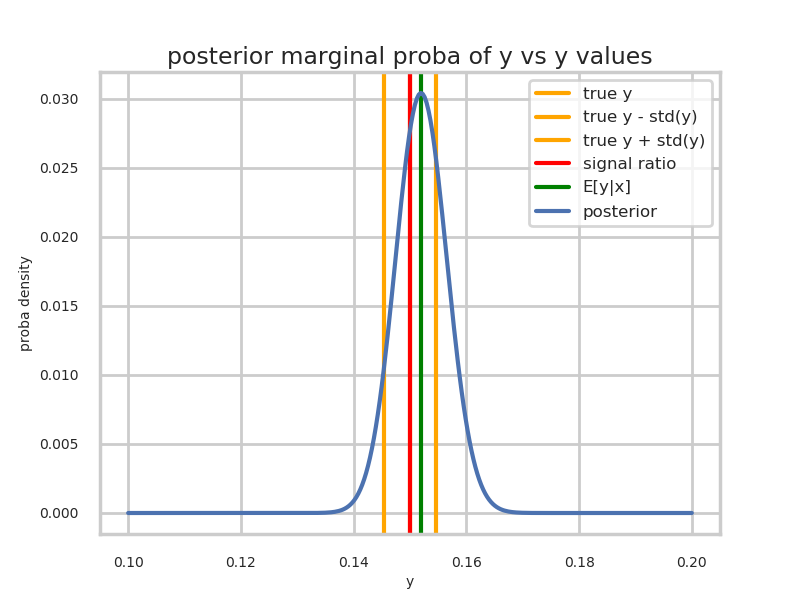
\includegraphics[width=\linewidth]{Chapter4/Figs/Raster/minitoy/marginal_y.png}
    \caption{$p(y|x)$}
    \label{fig:marginal_y}
  \end{subfigure}%
  \hfill
  \begin{subfigure}[t]{0.49\linewidth}
    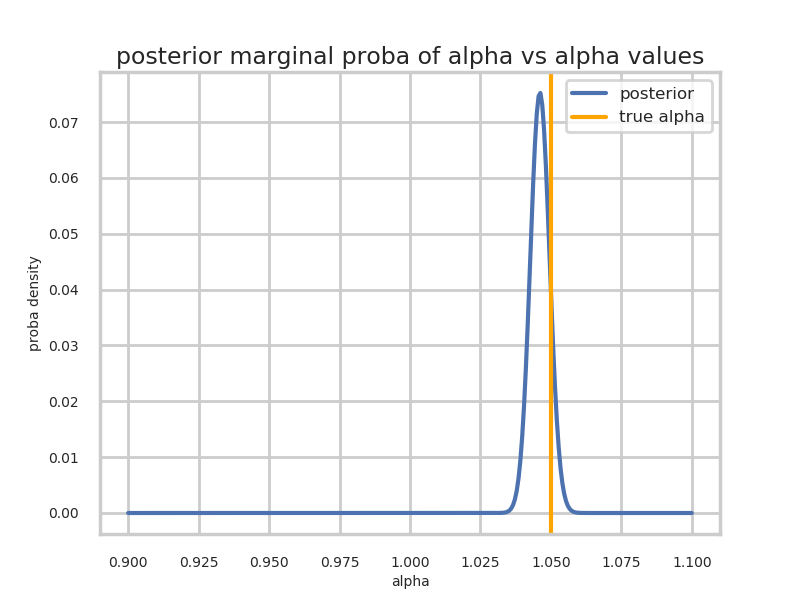
\includegraphics[width=\linewidth]{Chapter4/Figs/Raster/minitoy/marginal_alpha.png}
    \caption{$p(\alpha|x)$}
    \label{fig:marginal_alpha}
  \end{subfigure}
  \caption{Posterior probabilities for $y$ (left) and $\alpha$ (right)}
  \label{fig:marginals}
\end{figure}


Petit soucis ... L'erreur statistique et l'erruer systématique diminuent ensemble avec l'augmentation du nombre de donnée.
Plus on a de donnée meilleur est l'inférence sur $\alpha$.
Donc c'est normal !

Du coup j'ai vraiment du mal avec le concepte de l'erreur systématique qui ne diminue que doucement avec l'augmentation des données.

Si l'effet est invisible sur les données alors on a pas de problème.
Si l'effet est visible alors on peut contraindre + les paramètres de nuisance puisqu'on peut le mesurer !


\subsection{3D toy} % (fold)
\label{sub:3d_toy}

L'exemple jouet introduit dans \cite{DECASTRO2019170inferno} est un mélange de 2 processus (background \& signal)


Pour les backgrounds :
$$
f_b (x|r, \lambda) = \mathcal N \left ( (x_0, x_1) | (2+r, 0) 
\begin{bmatrix} 5 & 0 \\ 0 & 9 \end{bmatrix} \right ) Exp((x_2| \lambda)
$$


Pour les signaux :
$$
f_s (x|r, \lambda) = \mathcal N \left ( (x_0, x_1) | (1, 1) 
\begin{bmatrix} 1 & 0 \\ 0 & 1 \end{bmatrix} \right ) Exp((x_2| 2)
$$

Ce qui donne la vraissemblance :
$$
p(x | r, \lambda, \mu ) = (1-\mu) f_b(x|r, \lambda) + \mu f_s(x|r, \lambda)
$$

Ce toy a l'avantage d'être multidimensionnel et plus complexe que le précédent.


\begin{figure}[htb]
    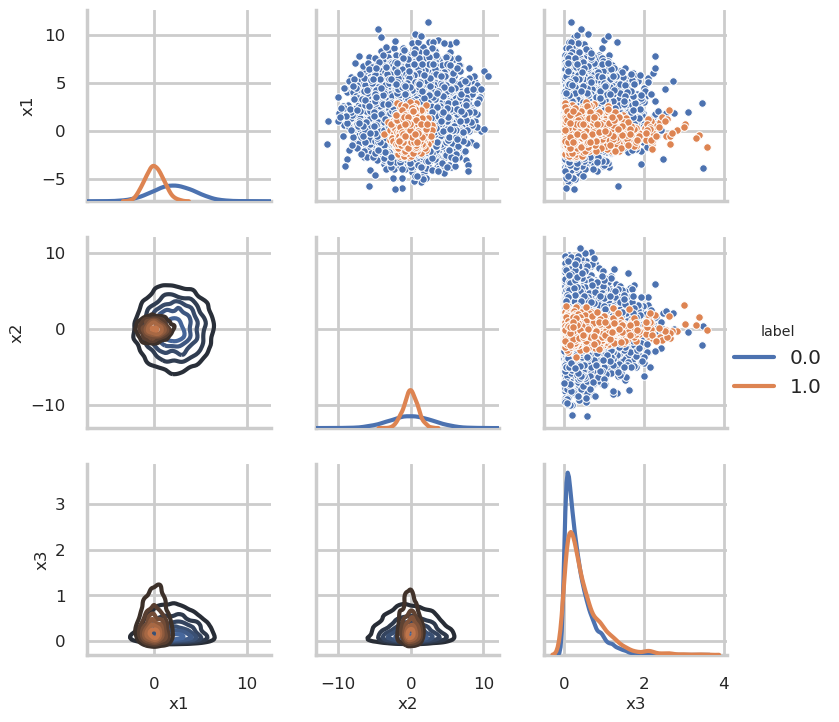
\includegraphics[width=\linewidth]{s3d2/pairgrid}
    \caption{Data distribution of the 3D toy}
    \label{fig:s3d2_pairgrid}
\end{figure}


Ici c'est le pompom l'erreur stat est minime et l'erreur systématique représente quasiment la totalité de l'erreur globale.


\begin{figure}[htb]
  \centering
  \begin{subfigure}[t]{0.49\linewidth}
    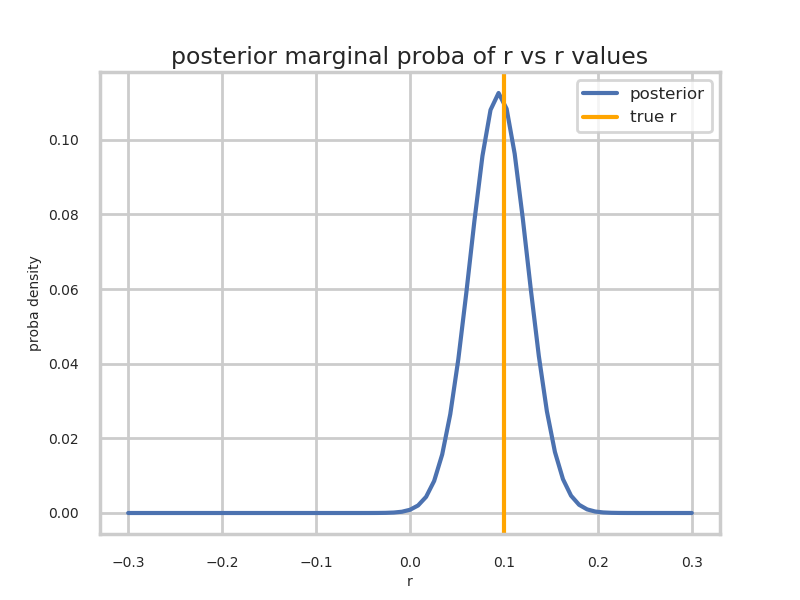
\includegraphics[width=\linewidth]{s3d2/marginal_r.png}
    \caption{$p(r|x)$}
    \label{fig:marginal_r}
  \end{subfigure}%
  \hfill
  \begin{subfigure}[t]{0.49\linewidth}
    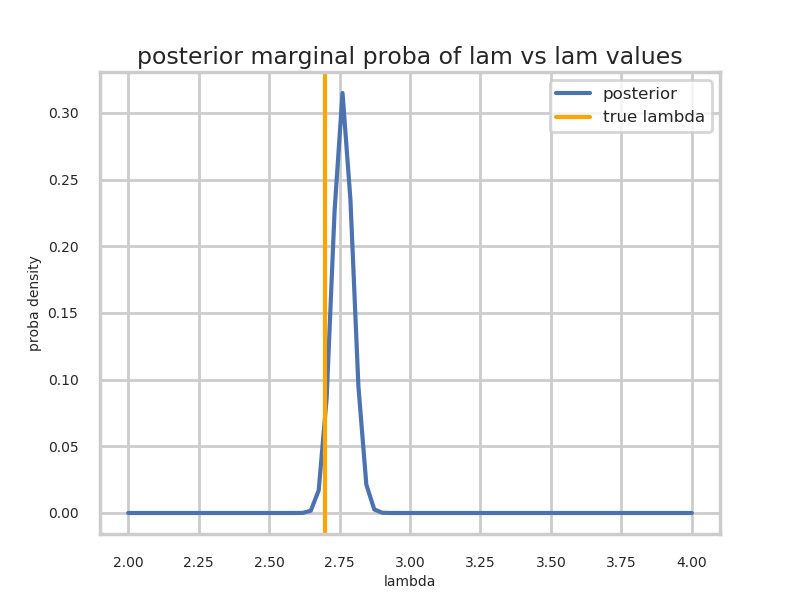
\includegraphics[width=\linewidth]{s3d2/marginal_lam.png}
    \caption{$p(\lambda|x)$}
    \label{fig:marginal_lambda}
  \end{subfigure}

  \begin{subfigure}[t]{0.49\linewidth}
    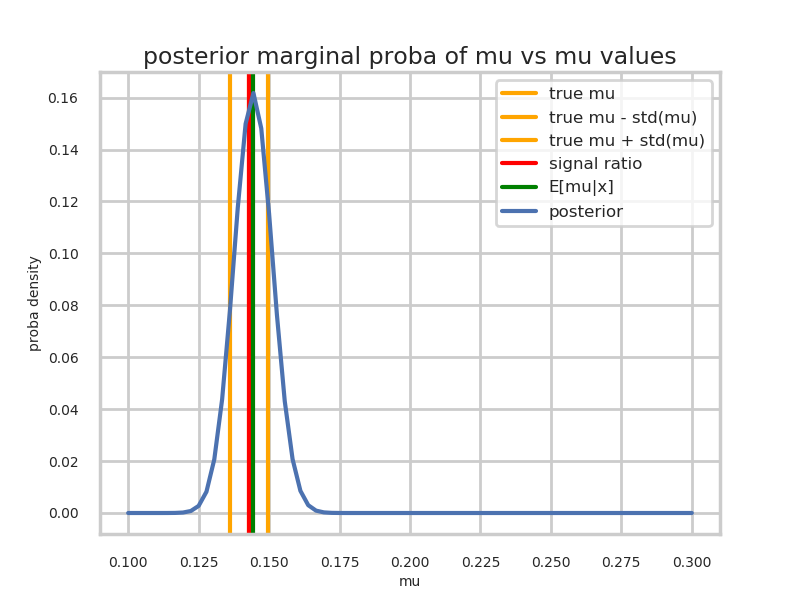
\includegraphics[width=\linewidth]{s3d2/marginal_mu.png}
    \caption{$p(\mu|x)$}
    \label{fig:marginal_mu}
  \end{subfigure}
  \caption{Posterior probabilities for $y$ (left) and $\alpha$ (right)}
  \label{fig:marginals}
\end{figure}


